% vim: filetype=tex spell

%Helmholtz Cage

\chapter{Helmholtz Cage}

\label{ch:Helmholtz}

The testing and calibration of the \ac{ACDS} it is required create a controllable, uniform magnetic field. The Helmholtz cage was constructed in 2009 by the \ac{ARC} mechanical team. The cage was designed to be able to create a 2~gauss magnetic field in any direction within the cage. This allows the Earth's magnetic field to be canceled out and the field inside to be equivalent to the Earth's field at any point above the Earth's surface.

\section{Hardware}

The cage Helmholtz consists of 3 pairs of perpendicular coils as shown in \cref{fig:helmholtz}. Each coil pair generates a nearly uniform magnetic perpendicular to the plane of the coil. Together the three perpendicular coil pairs can generated a field in any direction.

\begin{figure}[!ht]
    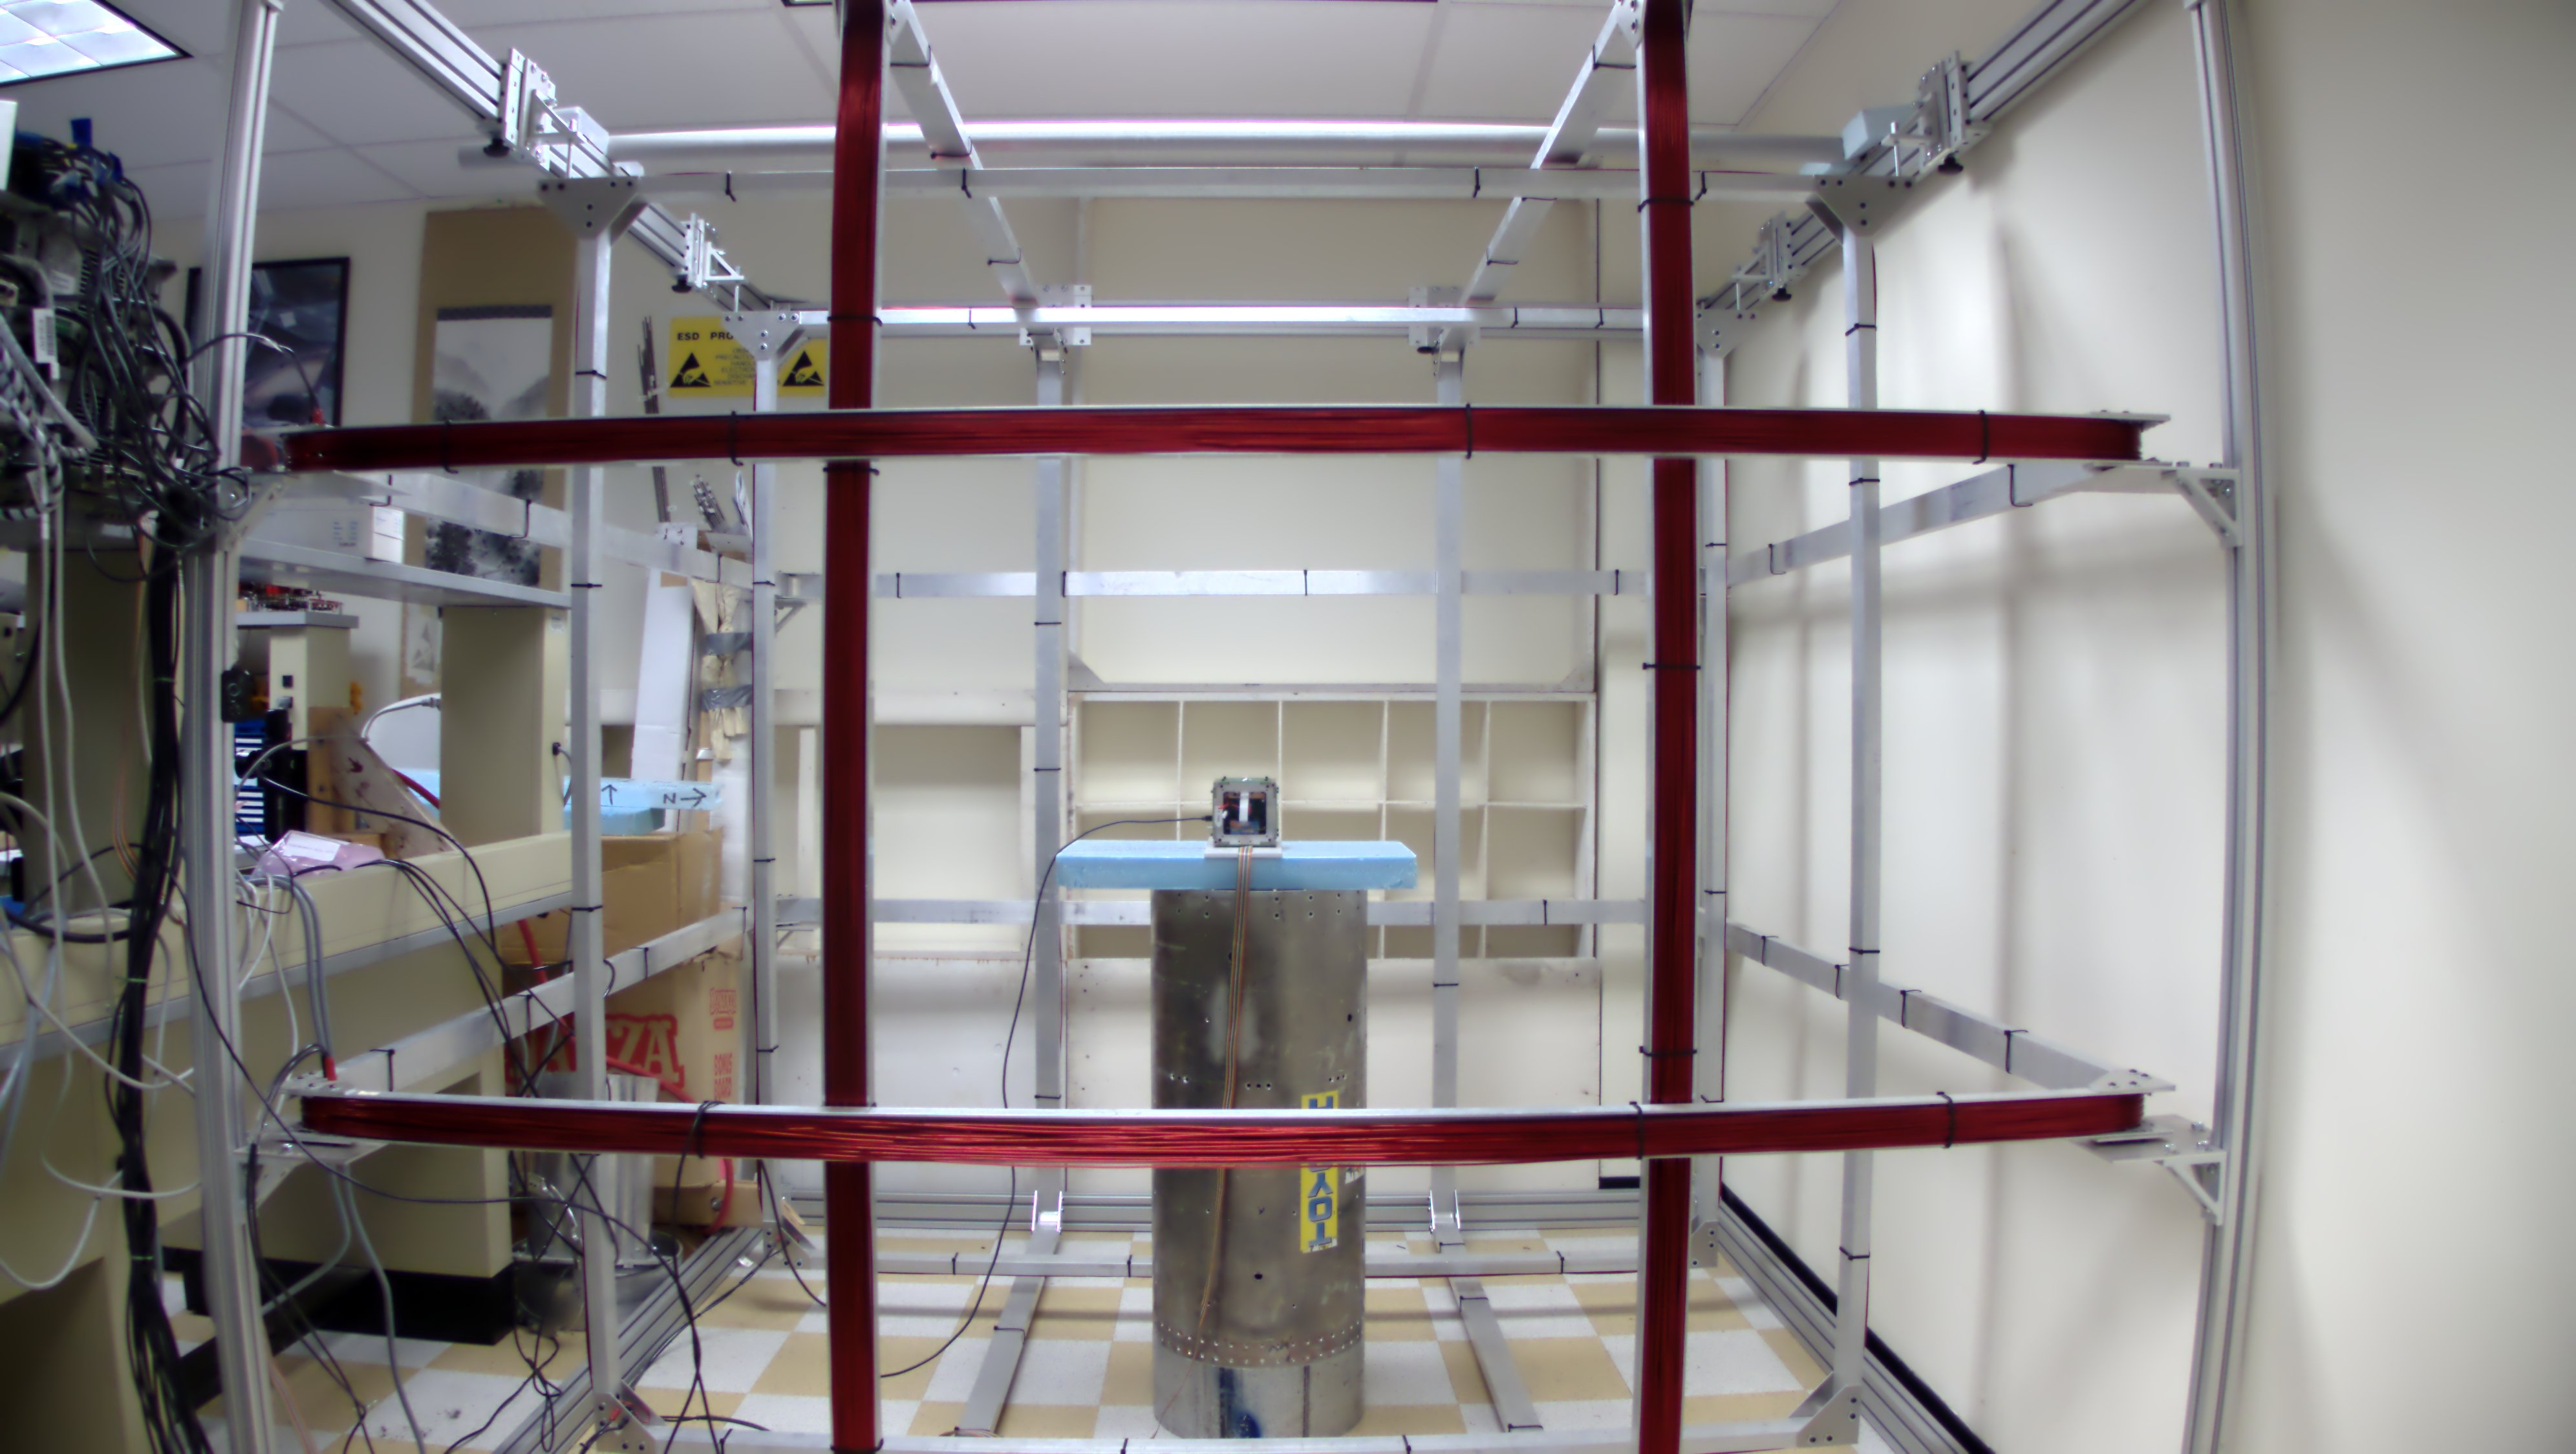
\includegraphics[width=\linewidth]{helmholtz-cage}
    \caption{The Helmholtz cage used for \acs{ACDS} testing}
    \label{fig:helmholtz}
\end{figure}

The coils are driven by a set of six Agilent E3633A power supplies as shown in \cref{fig:helmholtz-comp}. The power supplies have a maximum current of 20~A for output voltages less than 8~V or a maximum current of 10~A for output voltages of 20~V. The supplies are computer controlled with a \ac{GPIB} connection. 

Both coils in each pair require the same current to be driven in each coil to get a uniform field. This could be achieved by putting both coils in a pair in series but this would make the required voltage too large to be feasible. The coils could also be put in parallel but this requires the coils to be matched. The Helmholtz cage software sets the power supply currents to be the same for both coils in each pair.

An Alpha lab \#3AMG Milligauss Meter is used to measure the magnetic field of the Helmholtz cage. The meter is visible in \cref{fig:helmholtz-comp} to the left of the computer monitors. The Miligauss Meter has a digital display and an analog voltage output. The voltage output is read by a NI PCI-6010 Multifunction \ac{DAQ} installed in the Helmholtz cage computer.

\begin{figure}[!ht]
    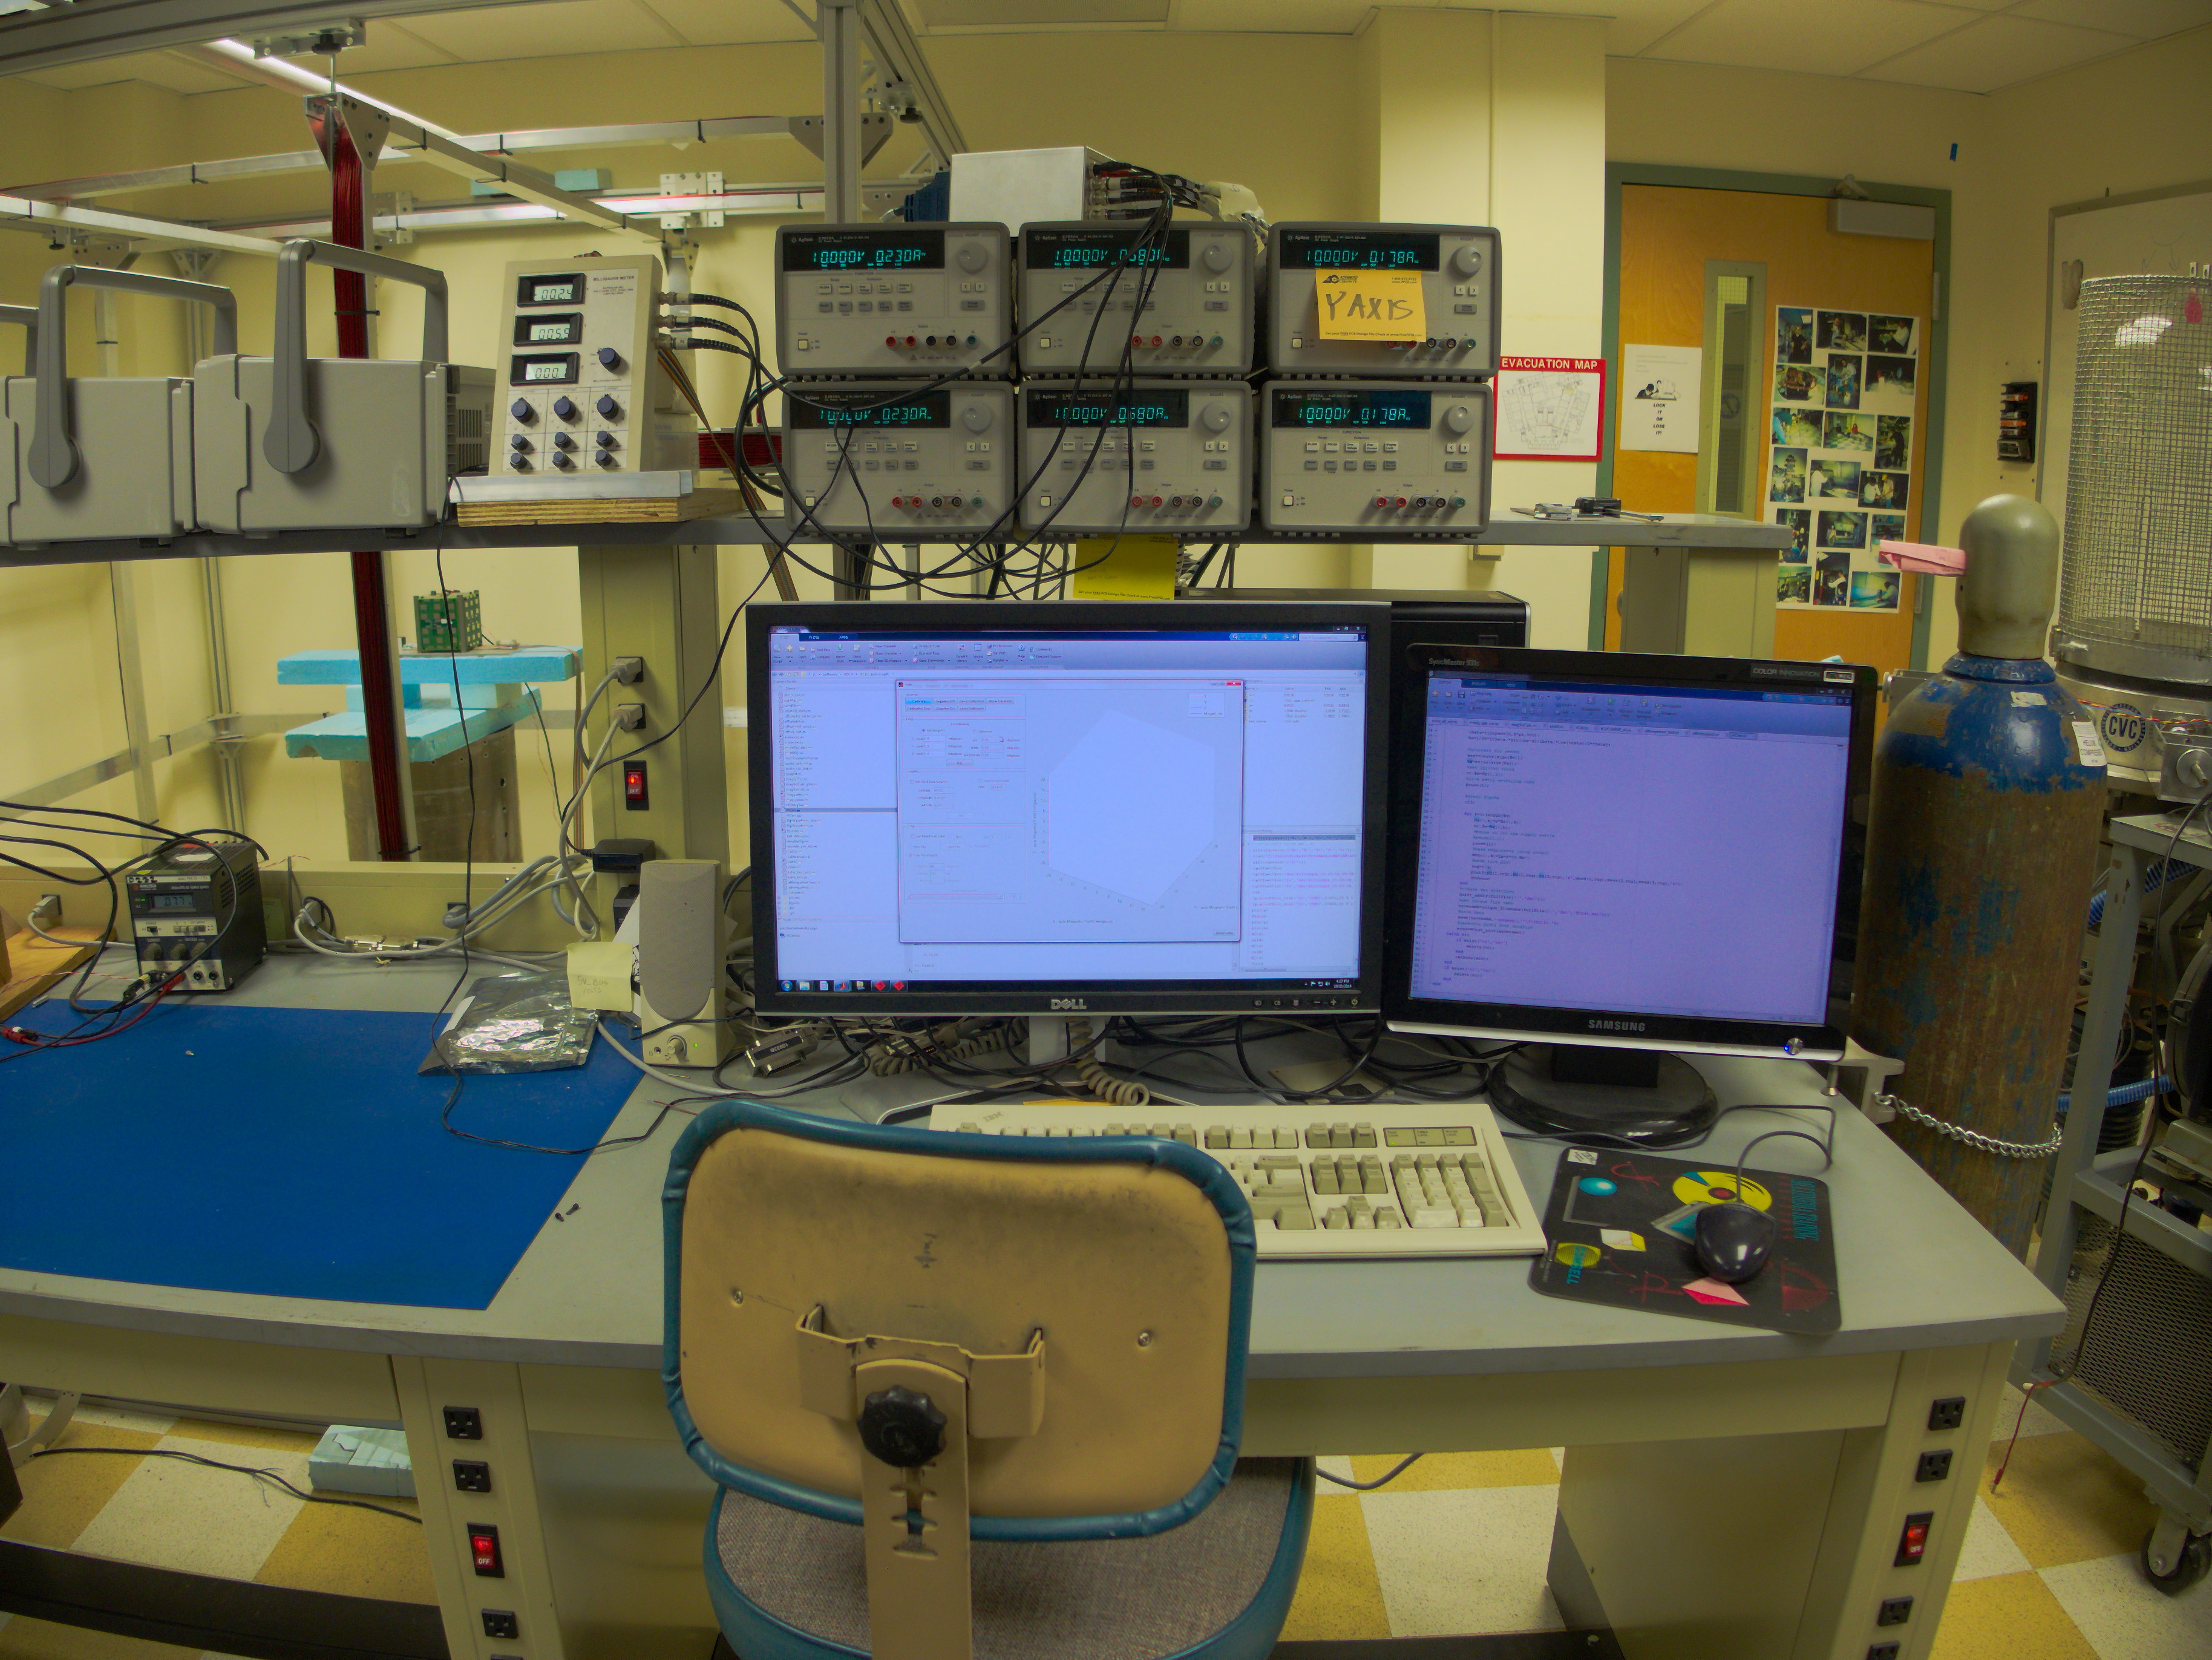
\includegraphics[width=\linewidth]{helmholtz-computer}
    \caption{The Helmholtz cage computer and power supplies}
    \label{fig:helmholtz-comp}
\end{figure}

\section{Software}

\Cref{fig:hc-block} shows the block diagram of the Helmholtz cage. The cage control class is a \matlab class that is used for low level interfacing to the Helmholtz cage hardware. The \ac{GPIB} interface is used to connect to the power supplies. The power supplies are connected to the coils through the H-bridge so that the current direction can be reversed. The H-bridge is controlled using the digital I\textbackslash{}O on the \ac{DAQ} card. The magnetometer is connected to the analog input channels of the \ac{DAQ} and reads the magnetic field in the Helmholtz cage. 

\begin{figure}[!ht]
    % We need layers to draw the block diagram
    \pgfdeclarelayer{background}
    \pgfdeclarelayer{foreground}
    \pgfdeclarelayer{Hardware}
    \pgfdeclarelayer{CPU}

    \pgfsetlayers{background,Hardware,CPU,main,foreground}

    \begin{tikzpicture}[node distance = 6mm, auto]
        \node[prog,text width=2.2cm]     (cc)    {cage\_control class};
        \node[perif,right=of cc]      (gpib)  {\rotatebox{90}{\acs*{GPIB}}};
        \node[perif,above=of cc]      (daq)   {\acs*{DAQ}};
        \node[hardware,right=of gpib] (ps)    {Power Supplies};
        \node[hardware,right=of ps]   (dir)   {H-bridge};
        \node[hardware,right=of dir]  (coils) {Helmholtz Coils};
        \node[hardware,above=of daq]  (mag)   {Three-axis Magnetometer};

        \node[prog,text width=2.2cm,left=of cc]       (user)   {User Application};

        \begin{pgfonlayer}{CPU}
            \node (push) at ([yshift=-1cm,xshift=-4mm]user.south west) {};
            \node[CPU,fit=(cc) (gpib) (daq) (push) (user)] (cpu) {};
            \node[above,anchor=south west] at (cpu.south west) {Helmholtz Cage Computer};
        \end{pgfonlayer}

        \path[dataL] (cc) -- (daq);
        \path[dataL] (daq) -- (mag);

        \path[dataL] (cc) -- (gpib);
        \path[dataL] (gpib) -- (ps);

        \path[dataL] (user) -- (cc);

        \path[powerL] (ps) -- (dir);
        \path[powerL] (dir) -- (coils);

        \path[phconn] (coils) |- (mag);
        \path[dataL] ([xshift=2mm]daq.north) -- ++(0,2mm) -| (dir);

    \end{tikzpicture}
    \caption{Helmholtz cage block diagram}
    \label{fig:hc-block}
\end{figure}

The feedback from the magnetometer is used to calibrate the Helmholtz cage. The cage is calibrated by setting the power supplies to a range of currents and reading back the magnetic field. The data is then used to compute a $4\times4$ transformation matrix, \lstMat{T}, to determine the current required to generate a given magnetic field. The magnetometer is not used in a closed loop fashion because magnetic fields produced by a device under test would change the magnetic field giving erroneous results.

The cage control class takes care of all of the low level hardware interaction and calibration for the Helmholtz cage. The cage control class opens interface objects to the power supplies and the \ac{DAQ}. The Helmholtz cage is controlled by setting properties of the class. Setting the \lstMat$Is$ property changes the current that the power supplies drive through the coils. The \lstMat$Bs$ property is a dependant property. Setting the \lstMat{Bs} property calculates the required currents using the calibration matrix \lstMat{T}, and sets \lstMat{Is}. Reading the \lstMat{Bs} property calculates the magnetic field setpoint using \lstMat{I} and \lstMat{T}. The read only \lstMat{Bm} property is also dependant as it represents the magnetic field read by the sensor. Reading \lstMat{Bm} causes the output voltage of the magnetometer to be read by the \ac{DAQ} and converted to a magnetic field reading.

\subsection{Compatibility}

The cage\_control class was originally developed on a 32-bit machine. When the code was moved to a 64-bit machine running \matlab R2011b the code did not work. This was because the cage\_control class uses the legacy interface for the \ac{DAQ} which is not supported in 64-bit \matlab. The 64-bit version of \matlab only supports the session-based interface which is the newer interface. The NI PCI-6010 is not usable with the session-based interface in \matlab R2011b to R2013b due to a known bug. The work around was to install 32-bit \matlab on the 64-bit machine which allowed the legacy interface to be used. The bug is supposedly fixed in \matlab R2014a so the cage\_control class could be ported to the session-based interface in the future.

\section{Testing}

The accuracy of the Helmholtz cage is important because it is used to measure the accuracy of the magnetometers on the CubeSat. The Helmholtz cage is not magnetically shielded so outside disturbances can affect the magnetic field in the cage.

To test the Helmholtz cage the commanded magnetic field was swept as shown in \cref{fig:hc-tst} and the field inside the cage was measured with the sensor. The measured field follows the commanded field for the most part but there are several areas where there is a visible difference between the measured and commanded field. 

\begin{figure}[htb]
    \centering
    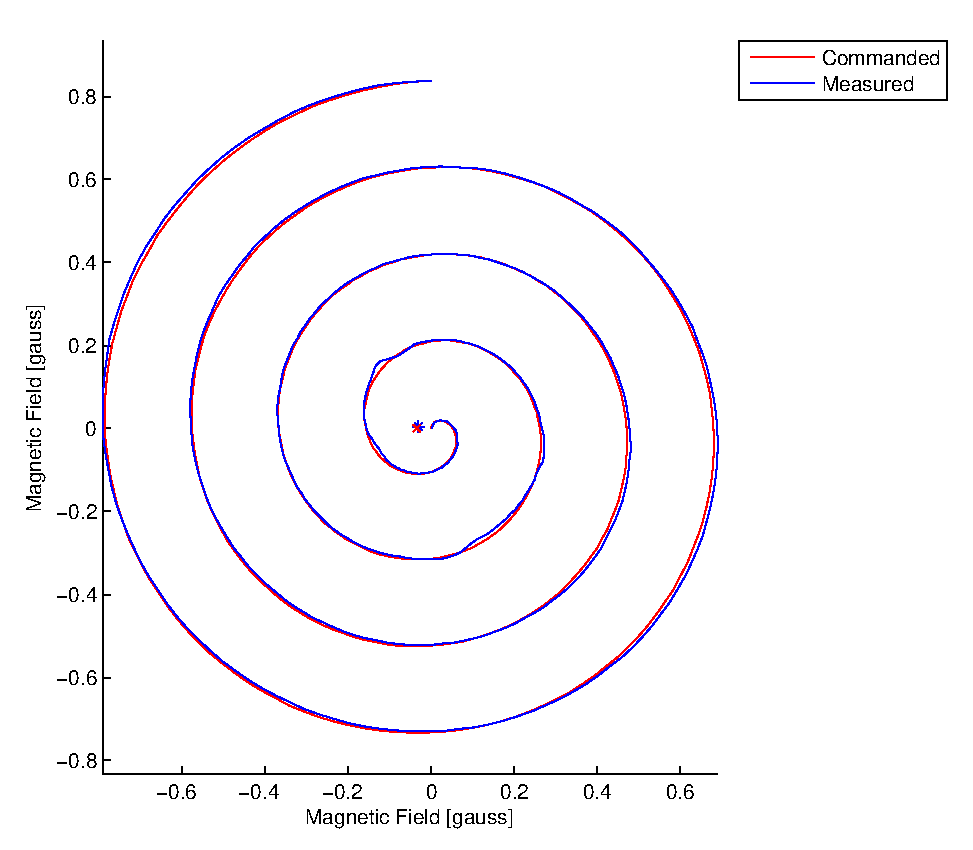
\includegraphics[width=0.8\linewidth]{HCtst}
    \caption{Helmholtz cage test field}
    \label{fig:hc-tst}
\end{figure}

\Cref{fig:hc-tst-err} shows the magnetic field error from the testing in \cref{fig:hc-tst}. The total RMS error for the plot is 9.4~mGauss. 

\begin{figure}[htb]
    \centering
    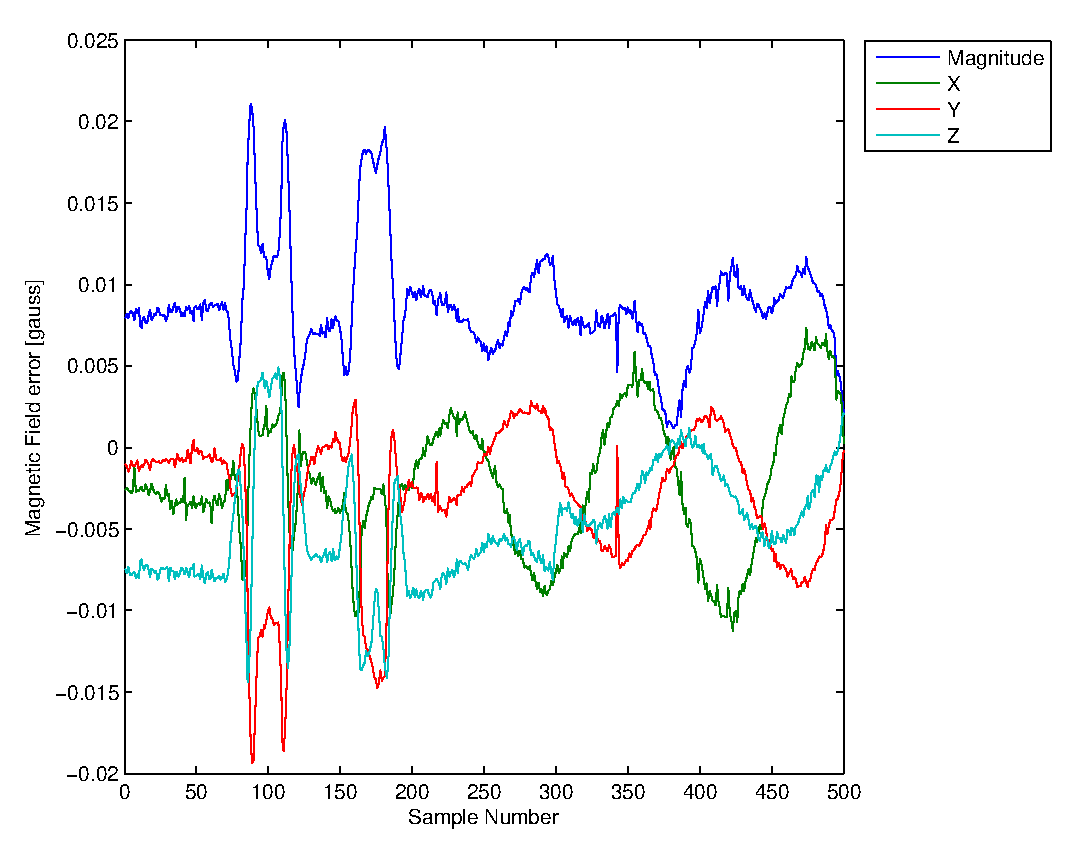
\includegraphics[width=\linewidth]{HCtst-error}
    \caption{Helmholtz cage test error}
    \label{fig:hc-tst-err}
\end{figure}

